% $Header$

% Template for presentation using Beamer LaTeX class. To use,
% download Beamer source from https://bitbucket.org/rivanvx/beamer/wiki/Home
% and copy to tex folder. This is usually found in your latex install
% directory, under a folder called "tex". Just look for other .cls files
% (for example, article.cls) and place the Beamer source similarly.

% Derived from "conference-ornate-20min.en.tex", found in 
% $INSTALL/beamer/solutions/conference-talks

% Original template copyright 2004 by Till Tantau <tantau@users.sourceforge.net>.
% Modification 2013 by Scott Boone <stboone@live.unc.edu>.
% No attribution or acknowledgement necessary. 

\documentclass{beamer}	% use beamer (presentation) class


% % % % % % % % % % % % % % % % % % BEAMER SETUP % % % % % % % % % % % % % % % % % % %
% Custom colors (from http://creative.unc.edu/resources/web-style-guide/color/)
\definecolor{carolinaBlue}{HTML}{56A0D3}
\definecolor{accessibilityBlue}{HTML}{5C8CBB}
\definecolor{backgroundColor}{HTML}{D9D9D9}
\definecolor{actionColor}{HTML}{4DB24C}

%\useoutertheme{sidebar}				% Insert sidebar w/navigation
\useoutertheme{infolines}				% Insert bar at bottom with author/title/page
\setbeamertemplate{headline}{} 			% remove the headline that infolines inserts

\setbeamercolor{background canvas}{bg=white}
\setbeamercolor*{structure}{fg=carolinaBlue}

\mode<presentation>
{
  \usetheme[height=12mm]{Rochester}

  \setbeamercovered{transparent}		% Handles transition transparency
}


% Add a logo to each page:
%\pgfdeclareimage[height=.5in]{university-logo}{unc_web_logos/large_blue_600px.png}
%\logo{\pgfuseimage{university-logo}}

% Or to the frame title:
\pgfdeclareimage[height=.5in]{university-logo}{unc_web_logos/medium_white_450px.png}
\addtobeamertemplate{frametitle}{}{
	\begin{textblock*}{100mm}(.75\textwidth,-1.25cm)
		\pgfuseimage{university-logo}
	\end{textblock*}
}

% % % % % % % % % % % % % % % % % % LOAD PACKAGES % % % % % % % % % % % % % % % % % % %

\usepackage{graphicx} 			% graphics support
\usepackage[utf8]{inputenc}		% font encoding
\usepackage{amssymb,amsmath} 	% math support
\usepackage[loadonly]{enumitem} 			% list customization
\usepackage{siunitx}			% SI unit support
%\usefonttheme{serif}			% Default is sans-serif.
\usepackage{textpos}			% Used for placement of logo.
\usepackage{datetime}			% Current date/time

\usepackage{lipsum} 			% insert lipsum text using \lipsum
\setlipsumdefault{1-31} 		% default lipsm paragraphs

\usepackage{natbib}				% uses natbib bibliography package...
								% cite using \citep for parenthetical...
								% cititations. 
								% See http://merkel.zoneo.net/Latex/natbib.php
								

\frenchspacing 					% omit extra spacing after periods

\newcommand{\pmt}{PM$_{2.5}$}	% '\pmt' is shortcut for PM2.5
\newcommand{\mmm}{\SI{}{\micro\metre}/m$^3$} % '\mmm' for ug/m3

% % % % % % % % % % % % % % % % DOCUMENT METADATA % % % % % % % % % % % % % % % % % % %

\title[Lorem Ipsum] % Short Title(optional, use only with long paper titles)
{Lorem Ipsum Dolor Sit Amet}	% Long Title (as listed in proceedings)

\subtitle
{Consectetur Adipisicing Elit, Sed Do Eiusmod Tempor} % Only if paper has subtitle

\author[Woody, Arunachalam] % (optional, use only with lots of authors)
{M.~Woody\inst{1,2} \and S.~Arunachalam\inst{1}}


\institute[UNC-CH] 				% (optional institutional information
								% used with \inst above)
{
  \inst{1}%
  Center for Environmental Modeling for Policy Development\\
  Institute for the Environment\\
  University of North Carolina at Chapel Hill
  \and
  \inst{2}%
  Department of Environmental Sciences and Engineering\\
  University of North Carolina at Chapel Hill
}

\date[\today]				% (or abbreviation of conference name)
{CMAS 2013}						% Full conference name

\subject{Atmospheric Modeling}	% only inserted into the PDF information catalog

% Delete this if you do not want the table of contents to pop up at
% the beginning of each subsection:
%\AtBeginSubsection[]
%{
%  \begin{frame}<beamer>{Outline}
%    \tableofcontents[currentsection,currentsubsection]
%  \end{frame}
%}

% If you wish to uncover everything in a step-wise fashion, uncomment
% the following command: 

%\beamerdefaultoverlayspecification{<+->}

% % % % % % % % % % % % % % DOCUMENT % % % % % % % % % % % % % % % % % % % % % % % % %

\begin{document}

\begin{frame}{~}						% Slide title goes in second brackets
										% use ~ on blank slides to preserve logo
\titlepage
\end{frame}

\begin{frame}{~}
  \tableofcontents						% can also add the option [pausesections]
\end{frame}

\section{Structure}
\begin{frame}{Structure}
	Create slides using the \texttt{frame} environment.
\end{frame}


\section{Layout}

\subsection{Figures}
\begin{frame}{Two figures}

\begin{figure}[ht]
	\begin{minipage}[b]{0.45\linewidth} 
		\centering
		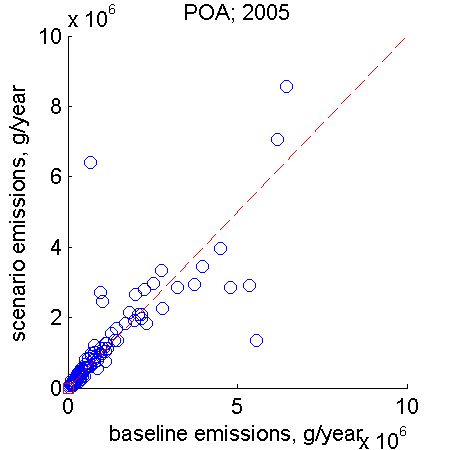
\includegraphics[width=\textwidth]{images/filename1}
		\caption{Caption text.}
		\label{fig:figure1}
	\end{minipage}
	\hspace{0.5cm}
	\begin{minipage}[b]{0.45\linewidth}
		\centering
		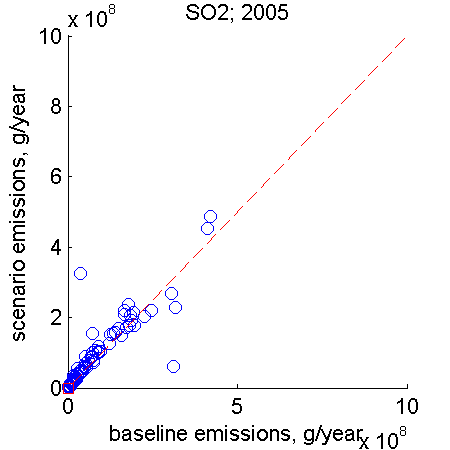
\includegraphics[width=\textwidth]{images/filename2}
		\caption{Other Caption Text.}
		\label{fig:figure2}
	\end{minipage}
\end{figure}

\end{frame}

\begin{frame}{Four figures}

\begin{figure}[ht]
	\begin{minipage}[t]{0.3\linewidth} 
		\centering
		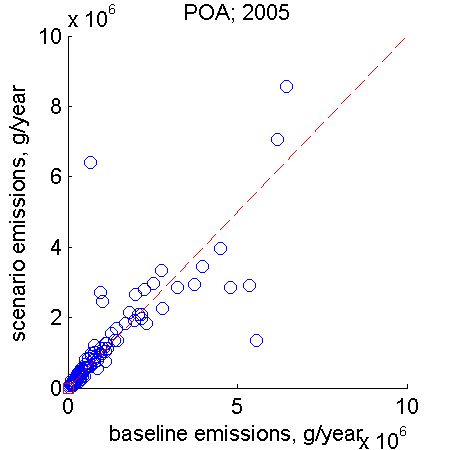
\includegraphics[width=\textwidth]{images/filename1}
	\end{minipage}
	\hspace{1cm}
	\begin{minipage}[t]{0.3\linewidth}
		\centering
		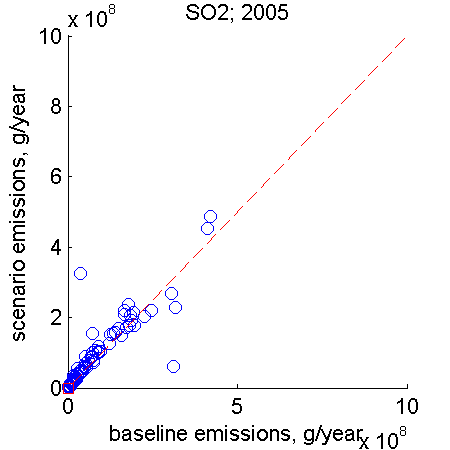
\includegraphics[width=\textwidth]{images/filename2}
	\end{minipage}\\
	
	\begin{minipage}[b]{0.3\linewidth} 
		\centering
		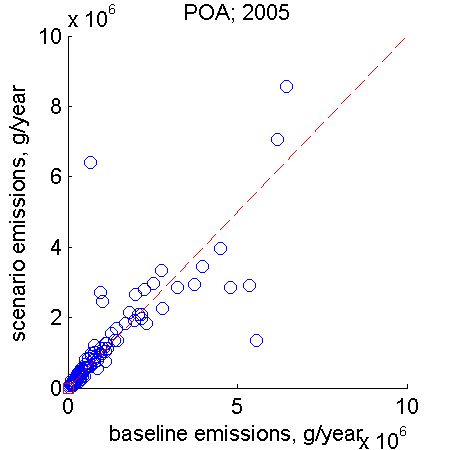
\includegraphics[width=\textwidth]{images/filename1}
	\end{minipage}
	\hspace{1cm}
	\begin{minipage}[b]{0.3\linewidth}
		\centering
		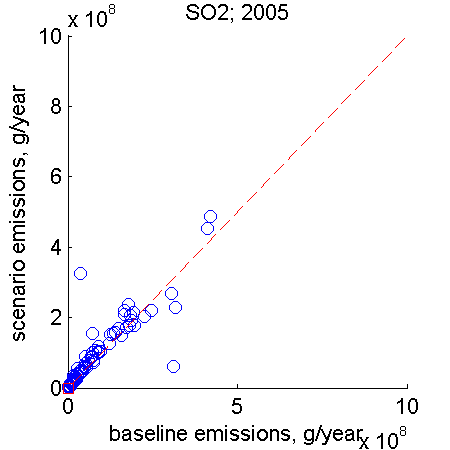
\includegraphics[width=\textwidth]{images/filename2}
	\end{minipage}
\end{figure}

\end{frame}

\subsection{Lists}

\begin{frame}{Lists.}{}
	\begin{itemize}
		\item Use \texttt{item} to separate, well, items.
		\item Especially if you have very short sentences or short phrases.
	\end{itemize}
\end{frame} 

\begin{frame}{Lists.}{Bullets}
	\begin{itemize}
		\item[--]Lists can have custom bullets.
		\item[Or Text:] \ldots Like so.
	\end{itemize}
\end{frame}

\begin{frame}{Lists.}{Numbers}
	\begin{enumerate}
		\item Or, you can use numbers.
		\item \ldots Like so.
	\end{enumerate}
\end{frame}

\section{Overlays}
\begin{frame}{Overlays.}

  You can create overlays\dots
  \begin{itemize}
  \item using the \texttt{pause} command:
    \begin{itemize}
    \item
      First item.
      \pause
    \item    
      Second item.
    \end{itemize}
  \end{itemize}
\end{frame}

\section{Equations}
\begin{frame}{Equations}

\begin{equation}
\nabla\cdot{\bf D} = \rho
\end{equation}

\begin{equation}
\nabla\cdot{\bf B} = 0
\end{equation}

\begin{equation}
\nabla\times{\bf E} = - {{\partial{\bf B}}\over{\partial t}}
\end{equation}

\begin{equation}
\nabla\times{\bf H} = {\bf J} + {{\partial{\bf D}}\over{\partial t}}
\end{equation}

\end{frame}



\section*{Using References}		% The asterisk keeps it out of the outline

\begin{frame}{Citations can be used as normal.}

  \begin{itemize}
  \item
    Statement~\citep{Box87}.
  \item
    Other statement~\citep{Ashok2013}.
  \item
    Another statement~\citep{Dun84}.
  \end{itemize}

\end{frame}


\section*{}
\subsection*{For Further Reading}		% This is all as normal--note use of 
										% [allowFramebreaks] to span multiple slides
\begin{frame}[allowframebreaks]
  \frametitle{References}
  \bibliographystyle{chicago}
  \bibliography{bibliography/bibliography-file}
 
\end{frame}

\end{document}


